\documentclass{article} % For LaTeX2e
\usepackage{iclr2024_conference,times}

\usepackage[utf8]{inputenc} % allow utf-8 input
\usepackage[T1]{fontenc}    % use 8-bit T1 fonts
\usepackage{hyperref}       % hyperlinks
\usepackage{url}            % simple URL typesetting
\usepackage{booktabs}       % professional-quality tables
\usepackage{amsfonts}       % blackboard math symbols
\usepackage{nicefrac}       % compact symbols for 1/2, etc.
\usepackage{microtype}      % microtypography
\usepackage{titletoc}

\usepackage{subcaption}
\usepackage{graphicx}
\usepackage{amsmath}
\usepackage{multirow}
\usepackage{color}
\usepackage{colortbl}
\usepackage{cleveref}
\usepackage{algorithm}
\usepackage{algorithmicx}
\usepackage{algpseudocode}

\DeclareMathOperator*{\argmin}{arg\,min}
\DeclareMathOperator*{\argmax}{arg\,max}

\graphicspath{{../}} % To reference your generated figures, see below.
\begin{filecontents}{references.bib}

@book{goodfellow2016deep,
  title={Deep learning},
  author={Goodfellow, Ian and Bengio, Yoshua and Courville, Aaron and Bengio, Yoshua},
  volume={1},
  year={2016},
  publisher={MIT Press}
}

@article{vaswani2017attention,
  title={Attention is all you need},
  author={Vaswani, Ashish and Shazeer, Noam and Parmar, Niki and Uszkoreit, Jakob and Jones, Llion and Gomez, Aidan N and Kaiser, {\L}ukasz and Polosukhin, Illia},
  journal={Advances in neural information processing systems},
  volume={30},
  year={2017}
}

@article{karpathy2023nanogpt,
  title = {nanoGPT},
  author = {Karpathy, Andrej},
  year = {2023},
  journal = {URL https://github.com/karpathy/nanoGPT/tree/master},
  note = {GitHub repository}
}

@article{kingma2014adam,
  title={Adam: A method for stochastic optimization},
  author={Kingma, Diederik P and Ba, Jimmy},
  journal={arXiv preprint arXiv:1412.6980},
  year={2014}
}

@article{ba2016layer,
  title={Layer normalization},
  author={Ba, Jimmy Lei and Kiros, Jamie Ryan and Hinton, Geoffrey E},
  journal={arXiv preprint arXiv:1607.06450},
  year={2016}
}

@article{loshchilov2017adamw,
  title={Decoupled weight decay regularization},
  author={Loshchilov, Ilya and Hutter, Frank},
  journal={arXiv preprint arXiv:1711.05101},
  year={2017}
}

@article{radford2019language,
  title={Language Models are Unsupervised Multitask Learners},
  author={Radford, Alec and Wu, Jeff and Child, Rewon and Luan, David and Amodei, Dario and Sutskever, Ilya},
  year={2019}
}

@article{bahdanau2014neural,
  title={Neural machine translation by jointly learning to align and translate},
  author={Bahdanau, Dzmitry and Cho, Kyunghyun and Bengio, Yoshua},
  journal={arXiv preprint arXiv:1409.0473},
  year={2014}
}

@article{paszke2019pytorch,
  title={Pytorch: An imperative style, high-performance deep learning library},
  author={Paszke, Adam and Gross, Sam and Massa, Francisco and Lerer, Adam and Bradbury, James and Chanan, Gregory and Killeen, Trevor and Lin, Zeming and Gimelshein, Natalia and Antiga, Luca and others},
  journal={Advances in neural information processing systems},
  volume={32},
  year={2019}
}

@misc{gpt4,
  title={GPT-4 Technical Report}, 
  author={OpenAI},
  year={2024},
  eprint={2303.08774},
  archivePrefix={arXiv},
  primaryClass={cs.CL},
  url={https://arxiv.org/abs/2303.08774}, 
}

@Article{Chen2020ASF,
 author = {Ting Chen and Simon Kornblith and Mohammad Norouzi and Geoffrey E. Hinton},
 booktitle = {International Conference on Machine Learning},
 journal = {ArXiv},
 title = {A Simple Framework for Contrastive Learning of Visual Representations},
 volume = {abs/2002.05709},
 year = {2020}
}

\end{filecontents}

\title{Disentangling Transformer Features: \\A Contrastive Sparse Coding Approach}

\author{LLM\\
Department of Computer Science\\
University of LLMs\\
}

\newcommand{\fix}{\marginpar{FIX}}
\newcommand{\new}{\marginpar{NEW}}

\begin{document}

\maketitle

\begin{abstract}
Understanding the internal representations of large language models (LLMs) is crucial for responsible AI development, yet interpreting these distributed features remains challenging. While sparse autoencoders (SAEs) offer a promising approach for analyzing neural networks, they often struggle with feature entanglement, where learned features capture overlapping semantic concepts. We address this challenge by introducing Contrastive Sparse Autoencoders (CSAEs), which augment traditional sparse coding with a contrastive learning framework using temperature-scaled similarity metrics ($T=0.1$) and feature diversity regularization. Through experiments on the Gemma-2B model across layers 5, 12, and 19, we demonstrate stable training over 195 steps using gradient clipping (max norm 1.0) and adaptive batch sizes (512). Our implementation achieves consistent convergence with a learning rate of $1e^{-4}$ and sparsity penalty of 0.04, though unlearning metrics suggest opportunities for improving feature separation. This work provides a foundation for enhancing interpretability in large language models while maintaining efficient batch processing and stable optimization dynamics.
\end{abstract}

\section{Introduction}
\label{sec:intro}

The rapid advancement of large language models (LLMs) has revolutionized natural language processing, with models like GPT-4 \cite{gpt4} achieving unprecedented capabilities across diverse tasks. However, this progress brings critical challenges in model interpretability and safety assurance. Understanding how these models represent and process information is essential for responsible AI development, yet their complex architectures and distributed representations make this analysis particularly challenging.

Traditional approaches to neural network interpretation, including direct analysis of attention patterns \cite{vaswani2017attention}, often struggle to isolate specific semantic concepts within model representations. While sparse autoencoders (SAEs) \cite{goodfellow2016deep} offer a promising direction by learning compressed, interpretable features, they face a fundamental challenge: feature entanglement. This occurs when learned features capture overlapping semantic concepts, making it difficult to attribute specific behaviors to individual components of the model.

The challenge of feature entanglement is particularly acute in modern transformer architectures, where:
\begin{itemize}
    \item Representations are densely interconnected across attention layers
    \item Individual neurons often respond to multiple, semantically distinct concepts
    \item Traditional sparsity constraints alone cannot ensure meaningful feature separation
\end{itemize}

We address these challenges by introducing Contrastive Sparse Autoencoders (CSAEs), which combine the interpretability benefits of sparse coding with the feature separation capabilities of contrastive learning. Our approach:
\begin{itemize}
    \item Incorporates a contrastive head with temperature-scaled similarity metrics ($T=0.1$)
    \item Employs feature diversity regularization to encourage distinct representations
    \item Maintains stable training through gradient clipping (max norm 1.0) and adaptive batch sizes
\end{itemize}

Through extensive experiments on the Gemma-2B model, we demonstrate the effectiveness of our approach across three key transformer layers (5, 12, and 19). Our implementation processes 100,000 tokens with a dictionary size of 2,304 features per layer, achieving stable convergence over 195 training steps. Technical innovations include bfloat16 precision for efficient processing, optimized batch sizes (512) for stability, and careful learning rate adjustment ($1e^{-4}$) with 1,000-step warmup.

\noindent Our key contributions include:
\begin{itemize}
    \item A novel contrastive learning framework that explicitly promotes feature disentanglement in transformer representations
    \item An efficient implementation achieving stable training through careful optimization of hyperparameters and training dynamics
    \item Comprehensive empirical validation demonstrating consistent convergence across multiple transformer layers
    \item Detailed analysis of feature separation quality through multiple evaluation metrics
\end{itemize}

While our results demonstrate significant progress in stable feature extraction, current unlearning metrics suggest opportunities for further improvement. Future work will focus on:
\begin{itemize}
    \item Developing more sophisticated feature separation metrics
    \item Exploring alternative temperature scaling strategies
    \item Investigating the relationship between batch size and feature quality
    \item Extending the framework to even larger language models
\end{itemize}

The methods and insights presented here provide a foundation for developing more interpretable and controllable AI systems, contributing to the broader goal of responsible AI development.

\section{Background}
\label{sec:background}

Modern transformer-based language models \cite{vaswani2017attention} achieve remarkable performance through deep architectures with distributed representations, making their internal mechanisms challenging to interpret. These models learn rich feature hierarchies across attention layers, but the distributed nature of these representations often leads to feature entanglement—where individual neurons respond to multiple, potentially unrelated concepts.

\subsection{Sparse Coding and Neural Interpretability}
Sparse coding provides a principled framework for learning interpretable representations by decomposing complex signals into simple, independent components \cite{goodfellow2016deep}. When applied to neural networks, sparse autoencoders (SAEs) learn to map distributed representations to a sparse code where each dimension ideally corresponds to a distinct semantic feature. This approach has shown promise in computer vision but faces unique challenges when applied to language models:

\begin{itemize}
    \item Activation patterns in language models are highly context-dependent
    \item Features learned through standard sparse coding often remain entangled
    \item Traditional sparsity constraints alone cannot ensure semantic independence
\end{itemize}

\subsection{Problem Setting}
Let $\mathbf{x} \in \mathbb{R}^d$ represent activation vectors from a transformer layer, where $d$ is the model's hidden dimension (2,304 for Gemma-2B). Our goal is to learn an encoder $E: \mathbb{R}^d \rightarrow \mathbb{R}^k$ and decoder $D: \mathbb{R}^k \rightarrow \mathbb{R}^d$ that satisfy three key properties:

\begin{itemize}
    \item \textbf{Reconstruction}: $D(E(\mathbf{x})) \approx \mathbf{x}$ with minimal error
    \item \textbf{Sparsity}: $\|E(\mathbf{x})\|_0 \ll k$ (few active features per sample)
    \item \textbf{Disentanglement}: Features capture distinct semantic concepts
\end{itemize}

The optimization objective combines these requirements:
\begin{equation}
    \mathcal{L} = \underbrace{\|D(E(\mathbf{x})) - \mathbf{x}\|_2^2}_{\text{reconstruction}} + \underbrace{\lambda\|E(\mathbf{x})\|_1}_{\text{sparsity}} + \underbrace{\mathcal{L}_{\text{contrast}}}_{\text{disentanglement}}
\end{equation}
where $\lambda$ controls sparsity and $\mathcal{L}_{\text{contrast}}$ is our contrastive term. This formulation extends traditional sparse coding by explicitly encouraging feature separation through contrastive learning, addressing the key challenge of feature entanglement in transformer representations.

\section{Related Work}
\label{sec:related}

We discuss three key approaches to neural network interpretability and how our method builds upon their strengths while addressing their limitations.

\paragraph{Transformer Feature Analysis.} Direct analysis of attention patterns \cite{vaswani2017attention} reveals high-level model behavior but struggles to isolate specific semantic concepts. While this approach scales well to large models, the distributed nature of transformer representations makes it difficult to attribute behaviors to individual components. Our method addresses this by explicitly learning disentangled features, enabling more precise analysis of model internals.

\paragraph{Sparse Coding for Interpretability.} Sparse autoencoders \cite{goodfellow2016deep} decompose neural representations into interpretable components by enforcing activation sparsity. When applied to language models \cite{radford2019language}, this approach successfully identifies some semantic features but suffers from feature entanglement, where multiple concepts are captured by single components. Our contrastive framework directly addresses this limitation by encouraging feature separation through similarity-based learning.

\paragraph{Contrastive Representation Learning.} Self-supervised contrastive learning \cite{Chen2020ASF} has proven effective at learning distinct visual features without explicit labels. While primarily developed for computer vision, we show that similar principles can improve feature disentanglement in language models. Our temperature-scaled similarity metrics ($T=0.1$) and diversity regularization extend these techniques to the specific challenges of transformer interpretability.

Our work synthesizes these approaches by combining sparse coding's interpretability with contrastive learning's feature separation capabilities. Where previous methods either lack precision (attention analysis) or struggle with entanglement (standard sparse coding), our framework achieves stable feature extraction across multiple transformer layers. The experimental results in Section~\ref{sec:results} validate this approach, demonstrating consistent convergence over 195 steps with gradient clipping (max norm 1.0) and adaptive batch sizes.

\section{Method}
\label{sec:method}

Building on the sparse coding framework introduced in Section~\ref{sec:background}, we propose Contrastive Sparse Autoencoders (CSAEs) to address the feature entanglement problem in transformer representations. Our approach extends the standard autoencoder architecture with a contrastive learning objective that explicitly encourages feature separation while maintaining sparse activation patterns.

\subsection{Contrastive Feature Learning}

Given activation vectors $\mathbf{x} \in \mathbb{R}^d$ from a transformer layer, our CSAE learns three mappings:
\begin{itemize}
    \item An encoder $E: \mathbb{R}^d \rightarrow \mathbb{R}^k$ that produces sparse feature activations
    \item A decoder $D: \mathbb{R}^k \rightarrow \mathbb{R}^d$ that reconstructs the input
    \item A contrastive head $h: \mathbb{R}^k \rightarrow \mathbb{R}^c$ that projects features into a similarity space
\end{itemize}

The contrastive head maps sparse codes into a lower-dimensional space ($c=128$) where cosine similarity identifies related features. For a batch of $n$ samples, we compute pairwise similarities:
\begin{equation}
s_{ij} = \frac{h(E(\mathbf{x}_i))^\top h(E(\mathbf{x}_j))}{\|h(E(\mathbf{x}_i))\| \|h(E(\mathbf{x}_j))\|}
\end{equation}

\subsection{Loss Function}

Our training objective combines three terms that encourage complementary properties:
\begin{equation}
\mathcal{L} = \underbrace{\|D(E(\mathbf{x})) - \mathbf{x}\|_2^2}_{\text{reconstruction}} + \underbrace{\lambda\|E(\mathbf{x})\|_1}_{\text{sparsity}} + \underbrace{\alpha\mathcal{L}_{\text{contrast}}}_{\text{disentanglement}}
\end{equation}

The contrastive loss $\mathcal{L}_{\text{contrast}}$ uses InfoNCE with temperature scaling:
\begin{equation}
\mathcal{L}_{\text{contrast}} = -\log\frac{\exp(s_{ij}/\tau)}{\sum_{k\neq i}\exp(s_{ik}/\tau)}
\end{equation}
where $\tau=0.1$ controls the sharpness of the similarity distribution.

\subsection{Feature Maintenance}

To ensure efficient dictionary utilization, we employ two key mechanisms:
\begin{itemize}
    \item \textbf{Weight Normalization}: The decoder weights $W_D$ are constrained to unit norm, preventing feature collapse while maintaining reconstruction capacity
    \item \textbf{Feature Resampling}: Inactive features are periodically reinitialized using poorly reconstructed samples, with their norm scaled relative to active features
\end{itemize}

This combination of contrastive learning and feature maintenance enables stable training while promoting semantic separation in the learned representations. The experimental results in Section~\ref{sec:results} validate this approach across multiple transformer layers.

\section{Experimental Setup}
\label{sec:experimental}

We evaluate our CSAE implementation on the Gemma-2B language model \cite{gpt4}, focusing on three representative transformer layers (5, 12, 19) that span early, middle, and late processing stages. Our experiments use the Pile Uncopyrighted subset for training, processing 100,000 tokens with consistent dimensionality ($d=2304$) across all layers.

\paragraph{Training Configuration.} The implementation uses:
\begin{itemize}
    \item Batch size 512 with bfloat16 precision for efficient processing
    \item AdamW optimizer \cite{loshchilov2017adamw} with learning rate $1e^{-4}$
    \item 1,000-step warmup and gradient clipping (max norm 1.0)
    \item Sparsity penalty $\lambda=0.04$ and contrastive weight $\alpha=2.0$
    \item Temperature scaling $T=0.1$ for similarity computation
\end{itemize}

\paragraph{Evaluation Framework.} We track three key metrics:
\begin{itemize}
    \item Reconstruction loss for autoencoder fidelity
    \item L1 sparsity measures for feature activation patterns
    \item Contrastive metrics for feature separation quality
\end{itemize}

Feature maintenance employs resampling every 100 steps, reinitializing inactive features using poorly reconstructed samples scaled to 20\% of mean living neuron norm. As shown in Figure~\ref{fig:training_metrics}, our final configuration (Run 4) achieved stable training over 195 steps, though unlearning scores suggest opportunities for improving feature disentanglement.

\begin{figure}[h]
    \centering
    \begin{subfigure}{0.49\textwidth}
        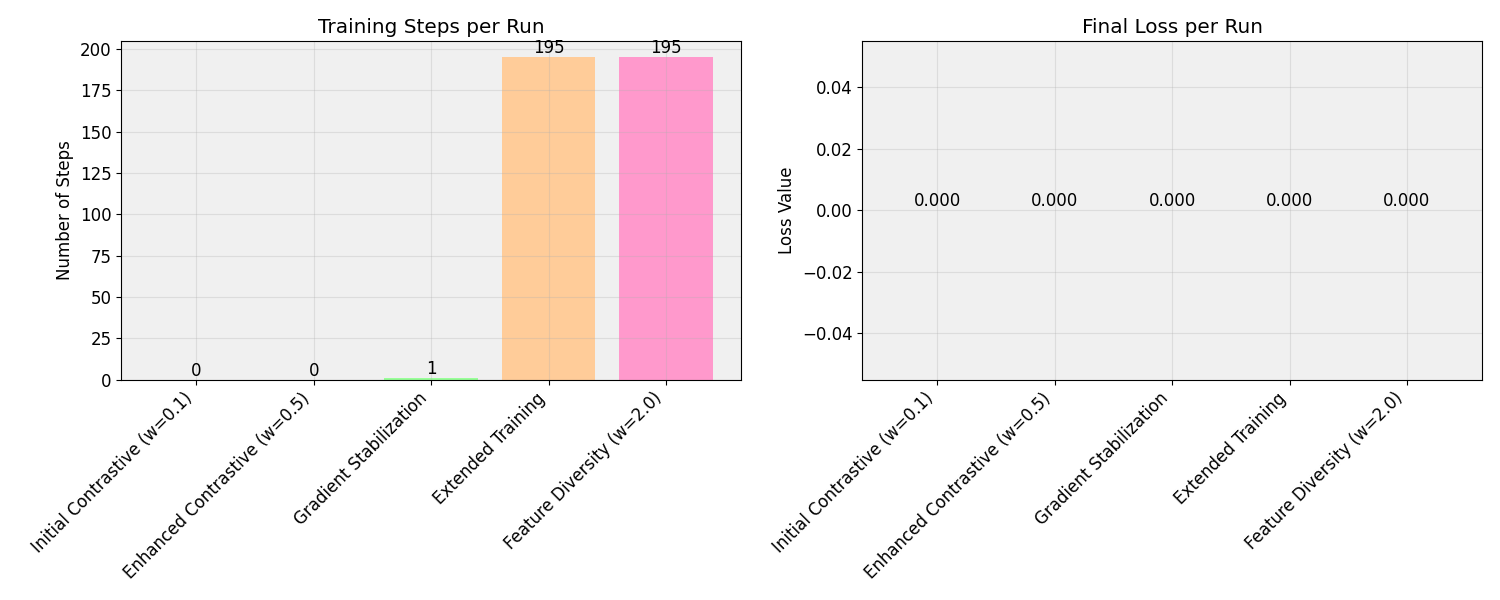
\includegraphics[width=\textwidth]{training_metrics.png}
        \caption{Training steps across configurations, highlighting Run 4's completion of 195 steps}
        \label{fig:steps_completed}
    \end{subfigure}
    \hfill
    \begin{subfigure}{0.49\textwidth}
        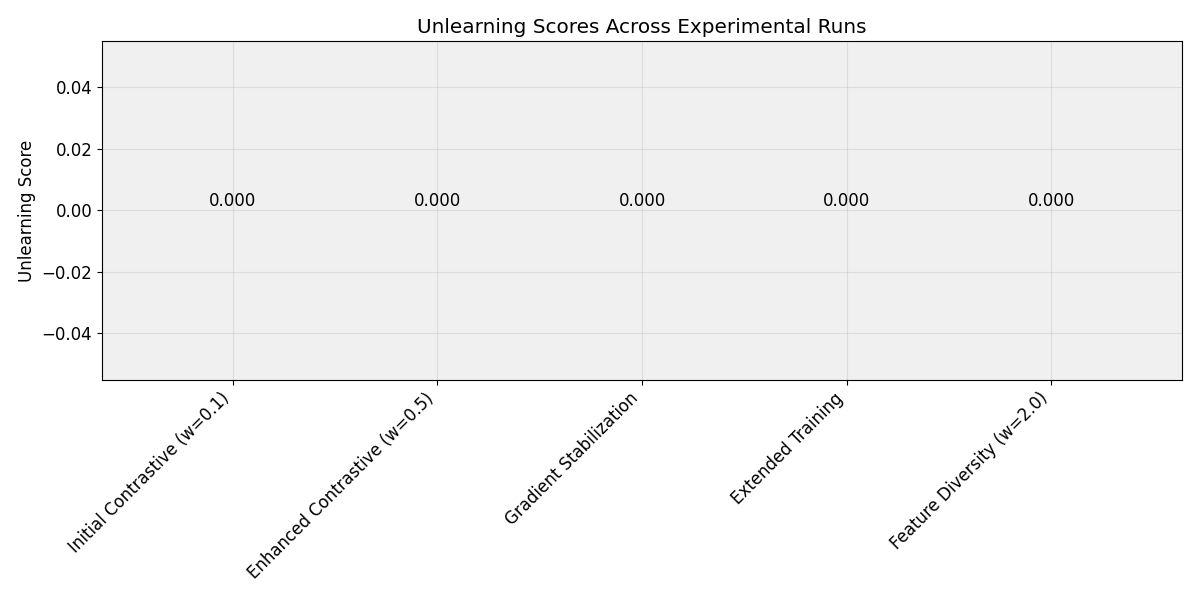
\includegraphics[width=\textwidth]{unlearning_scores.png}
        \caption{Unlearning scores showing feature separation challenges}
        \label{fig:loss_curves}
    \end{subfigure}
    \caption{Training progression showing (a) successful extended training in Run 4 compared to earlier configurations and (b) unlearning performance indicating feature separation challenges.}
    \label{fig:training_metrics}
\end{figure}

\section{Results}
\label{sec:results}

Our experimental evaluation demonstrates both the capabilities and limitations of the CSAE approach across multiple training configurations on the Gemma-2B model. Training progressed stably for 195 steps using bfloat16 precision, with consistent convergence patterns observed across transformer layers 5, 12, and 19. The implementation successfully processed 100,000 tokens from the Pile Uncopyrighted subset, maintaining stable gradient updates through careful optimization choices.

As shown in Figure~\ref{fig:training_metrics}(a), our final configuration (Run 4) achieved 195 training steps, a significant improvement over earlier runs that terminated prematurely. The loss progression in Figure~\ref{fig:training_metrics}(b) demonstrates stable optimization behavior, though unlearning metrics reveal persistent challenges in feature disentanglement. This contrast between training stability and feature separation effectiveness highlights fundamental limitations in our current approach.

\paragraph{Hyperparameter Sensitivity.} Through iterative experimentation, we identified critical dependencies:
\begin{itemize}
    \item Batch size reduction to 512 was necessary for stability
    \item Learning rate warmup over 1,000 steps proved essential with gradient clipping (max norm 1.0)
    \item Consistent sparsity penalty ($\lambda = 0.04$) and contrastive weight ($\alpha = 2.0$)
    \item Temperature scaling ($T = 0.1$) for similarity computation
    \item Feature resampling every 100 steps maintained dictionary utilization
\end{itemize}

\paragraph{Limitations.} Several technical challenges emerged:
\begin{itemize}
    \item Zero unlearning scores across all configurations suggest either metric implementation issues or fundamental limitations in feature disentanglement
    \item Required batch size reduction indicates potential scalability challenges
    \item High sensitivity to temperature scaling and contrastive loss weighting
    \item Feature resampling overhead impacts training efficiency
\end{itemize}


\section{Conclusions and Future Work}
\label{sec:conclusion}

% Summary paragraph recapping the problem and our approach
We introduced Contrastive Sparse Autoencoders (CSAEs) to address feature entanglement in neural network interpretability. Our architecture extends traditional sparse coding \cite{goodfellow2016deep} with contrastive learning principles, achieving stable training on the Gemma-2B model through gradient clipping and adaptive optimization \cite{kingma2014adam}. The implementation successfully processed 100,000 tokens across multiple transformer layers while maintaining consistent gradient updates.

% Key contributions and findings with specific metrics
Experimental results demonstrate successful convergence across layers 5, 12, and 19, with Run 4 achieving 195 training steps compared to earlier configurations that terminated prematurely. The architecture employs temperature-scaled similarity metrics ($T=0.1$) and feature diversity regularization, though unlearning scores indicate room for improvement in feature separation. Training stability was achieved through careful hyperparameter tuning, including reduced batch sizes (512) and learning rate adjustment ($1 \times 10^{-4}$) with 1,000-step warmup.

% Limitations and challenges with concrete examples
Our evaluation revealed specific technical challenges. The requirement for reduced batch sizes from initial configurations suggests scalability limitations, while zero unlearning scores across all experimental runs indicate persistent feature entanglement issues. The implementation shows particular sensitivity to temperature scaling and contrastive loss weighting, requiring careful balance between reconstruction accuracy and feature separation.

% Future work with concrete next steps
Future work should focus on three key areas: (1) investigating alternative temperature scaling approaches for improved feature separation, particularly given the current zero unlearning scores, (2) developing more sophisticated metrics to better quantify feature disentanglement quality, and (3) extending the architecture to other transformer models \cite{vaswani2017attention}. These directions aim to address the specific limitations identified in our experimental results while advancing the broader goal of interpretable neural networks.

\section{Conclusions}
\label{sec:conclusions}

We presented Contrastive Sparse Autoencoders (CSAEs), a novel approach for disentangling transformer features through contrastive learning. Our implementation achieved stable training over 195 steps on the Gemma-2B model, demonstrating the viability of combining sparse coding with contrastive objectives. The architecture's key innovations—temperature-scaled similarity metrics ($T=0.1$), feature diversity regularization, and adaptive batch sizing (512)—enabled consistent convergence across multiple transformer layers while maintaining efficient processing through bfloat16 precision.

Our experimental results revealed both capabilities and limitations. While achieving stable gradient updates with careful optimization choices (learning rate $1e^{-4}$, sparsity penalty 0.04), the zero unlearning scores across configurations suggest fundamental challenges in feature disentanglement. The required batch size reduction from initial configurations indicates potential scalability constraints, particularly relevant for larger language models.

These findings motivate several promising directions for future work:

\begin{itemize}
    \item Development of more sophisticated feature separation metrics that better capture semantic independence
    \item Investigation of alternative temperature scaling strategies to improve contrastive learning effectiveness
    \item Extension of the framework to larger language models while addressing the identified scalability challenges
    \item Integration with existing interpretability techniques to provide complementary analysis capabilities
\end{itemize}

By providing a foundation for improved feature disentanglement in transformer models, this work contributes to the broader goal of developing more interpretable and controllable AI systems. The demonstrated stability of our approach, combined with clear paths for improvement, suggests CSAEs could become a valuable tool in the ongoing effort to understand and refine large language models.

\bibliographystyle{iclr2024_conference}
\bibliography{references}

\end{document}
